\documentclass[10pt,a4paper]{article}
\usepackage[utf8]{inputenc}
\usepackage[italian]{babel}
\usepackage{amsmath}
\usepackage{amsfonts}
\usepackage{amssymb}
\usepackage{graphicx}
\usepackage{gensymb}
\usepackage[left=2cm,right=2cm,top=2cm,bottom=2cm]{geometry}
\newcommand{\rem}[1]{[\emph{#1}]}

\author{Gruppo BN \\ Lisa Bedini, Federico Belliardo, Marco Costa}
\title{Esperienza 14: misura del coefficiente di assorbimento del Mylar tramite Lock-in}
\begin{document}

\maketitle
\section{Scopo dell'esperienza}
Questa esperienza è finalizzata alla misura della costante di assorbimento del Mylar. Nella prima parte ci si propone di montare i circuiti e caratterizzarne il singolo funzionamento, successivamente procederemo a collegarli fra loro per eseguire la misura mediante Lock-in.

\section{Materiale occorrente}
\begin{itemize}
\item TL082 (JFET input dual Op-Amp);
\item 4 TL081 (JFET input Op-Amp);
\item SN7400 (4 porte NAND);
\item DG441 (4 interruttori analogici CMOS);
\item 2N1711/BC182 (transistor NPN);
\item LED rosso;
\item fotodiodo;
\end{itemize}

Tutte le resistenze, i condensatori, le tensioni di alimentazione e la tensione in uscita dal Lock-in sono stati misurati con il multimetro digitale (in DC), quindi l'errore è stato propagato secondo le specifiche nel manuale ($0.8\% + 3\,\mbox{digit}$ per le resistenze,$4\% + 3\, \mbox{digit}$  per i condensatori, $0.5\% + 1\,\mbox{digit}$ per i voltaggi). I tempi e le restanti tensioni sono state misurate con i cursori dell'oscilloscopio: l'errore sui tempi è dato dalla risoluzione dei cursori stessi mentre quello sulle tensioni è stato propagato considerando sia l'errore sul posizionamento dei cursori sia l'errore sistematico del $3\%$.

\section{Schema a blocchi}
Il circuito Lock-in è usato per effettuare misure di segnali deboli in un ambiente molto rumoroso. Nel nostro caso il segnale è la luce emessa dal LED. Tale segnale non è continuo ma modulato da un' onda sinusoidale prodotta dal generatore di funzioni. Abbiamo impostato una frequenza pari a $1\,\mbox{kHz}$ per eliminare il rumore \emph{1/f} dovuto alla presenza di dispositivi attivi\footnote{Può essere prodotto dalle discontinuità intrinseche dei materiali costruttivi.}. In figura \ref{fig:schemablocchi} si nota come questo circuito complesso sia costituito da sottocircuiti (che saranno analizzati e spiegati successivamente); in particolare nella parte superiore dello schema si trovano i circuiti che servono a sfruttare sia la parte positiva che negativa del segnale per la misura, mentre nella parte inferiore si trovano i circuiti di amplificazione del segnale da misurare.

\begin{figure}[!htb]
  \centering
  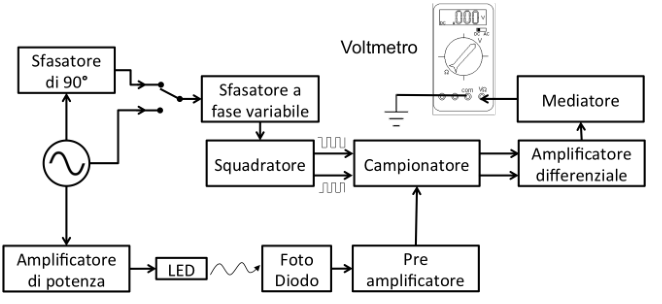
\includegraphics[scale=0.75]{schemablocchi.png}
\caption{Schema a blocchi del circuito Lock-in.\label{fig:schemablocchi}}
\end{figure}


\section{Implementazione schema a blocchi}

\subparagraph{Amplificatore di potenza e preamplificatore}
Abbiamo montato il circuito in figura \ref{fig:ampli-preampli} inviando a S1 un'onda sinusoidale di ampiezza picco-picco pari a $V_{pp}= 5.92\pm0.03 \,\mbox{V}$ e frequenza $f=1.03\pm0.01\,\mbox{kHz}$. 

Il circuito consiste in un amplificatore di potenza realizzato con un transistor NPN. Tale transistor è
dotato di circuito di polarizzazione che riceve in ingresso il segnale dal generatore di funzioni, che controlla la corrente di base, quindi l'intensità luminosa. Nella seconda parte, elettricamente separata dalla prima, troviamo il  circuito di lettura del fotodiodo, che a causa dell'OpAmp presenta un alta impedenza di ingresso e bassa impedenza di uscita e permette quindi di osservare la risposta del diodo senza alterarla.%dovrebbe esse un amplificatore a transimpedenza
Il segnale del fotodiodo è successivamente derivato per ottenere un segnale a media nulla, quindi inviato all'amplificatore non invertente dal guadagno di circa $A = 30$.\\ 

\subparagraph{Misura della costante di assorbimento senza Lock-in}
Il circuito è sensibile alla luce ambientale, quindi abbiamo posto particolare attenzione a questo fatto durante la presa dati. %ceeeerto...ci si mette questa cosa o no? direi di no
All'uscita S6 si ottiene la forma d'onda sinusoidale in figura \ref{fig:S6} che ha ampiezza $V=3.26\pm0.05\,\mbox{V}$. Si nota che questa tensione è affetta da rumore a bassa frequenza, probabilmente dovuto all'illuminazione ambientale, pertanto l'errore su tali misure sarà maggiore di quello strumentale.
%forse meglio dire come podo, errore 1\%? Dovremmo dire come abbimo effettuato le misure dato che c'è un evidente problema di rumore che modula. Da lì dovremmo poi stabilire quale errore abbiamo preso. 
Abbiamo ripetuto la misura della tensione in uscita in funzione del numero $n$ di lastrine di Mylar poste fra LED e fotodiodo, i dati sono rappresentati in tabella \ref{tab:abs1}. 

E' noto l'andamento teorico della tensione: $V_{out}=V_0 exp(-n/n_0)$. Abbiamo eseguito sia un fit esponenziale  sia logaritmico del tipo $ln(V_{out})=b-\frac{n}{a}$ (così da fittare una retta in carta logaritmica). Dal fit esponenziale (vedi grafico a sinistra in figura\ref{plot1}) si ottengono $n_0=3.44\pm0.04$, $V_0=5.74\pm0.09\,\mbox{V}$ e un $\chi^2 _{rid}=600$\footnote{Probabilmente dovuto a una sottostima dell'errore.}; da questi dati, sapendo che lo spessore di ogni lastrina è pari a $150\mu \mbox{m}$ si ottiene la lunghezza caratteristica di assorbimento $x_{ass}=0.52\pm0.01\,\mbox{mm}$. Dal fit lineare (vedi grafico a destra in figura \ref{plot1}) si ottengono $a=-0.174\pm0.003$ e $b=1.24\pm0.02$ con un $\chi^2_{rid}=7.6$; quindi $V_0= 3.46\pm0.06\,\mbox{V}$ e $n_0=5.7\pm0.1$ e $x_{ass}=0.86\pm0.01\,\mbox{mm}$.

%dato il chi^2 metterei solo il lineare. Ok, d'accordo: se non mettiamo offset nel fit esponenziale è inutile mettere tutti e due

\begin{figure}[!htb]
  \centering
  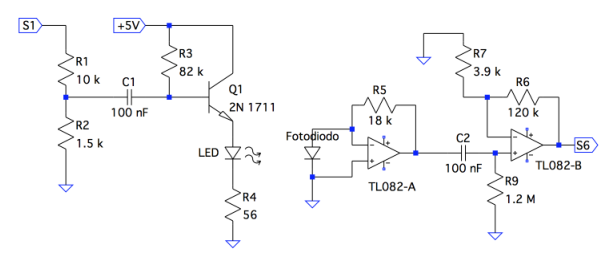
\includegraphics[scale=0.75]{ampli-preampli.png}
\caption{Schema a blocchi del circuito Lock-in.\label{fig:ampli-preampli}}
\end{figure}

\begin{figure}[!htb]
  \centering
  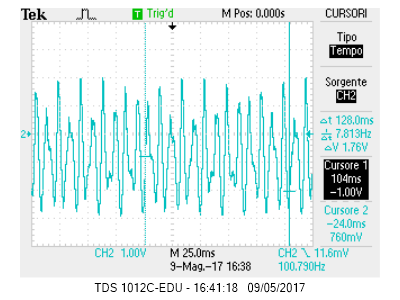
\includegraphics[scale=0.75]{S6.png}
\caption{Onda in S6; si nota che il segnale presenta rumore a bassa frequenza.\label{osc:S6}}
\end{figure}

\begin{table}[!htb]
\centering
\begin{tabular}{|c|c|c|}
\hline
n	&	$V_{out}\,\mbox{[V]}$	&	$\Delta V\,\mbox{[V]}$\\
\hline
0 &  3.26  &  0.05\\
\hline
1  & 2.96  &  0.05\\
\hline
2 &  2.48  &  0.05\\
\hline
3  & 2.12   & 0.04\\
\hline
4   &1.82   & 0.04\\
\hline
5   &1.55    &0.04\\
\hline
6   &1.17   & 0.03\\
\hline
7   &0.95    & 0.02\\
\hline
\end{tabular}
\caption{Presa dati della tensione in S6.\label{tab:abs1}}
\end{table}

\begin{figure}[!htb]
  \centering
  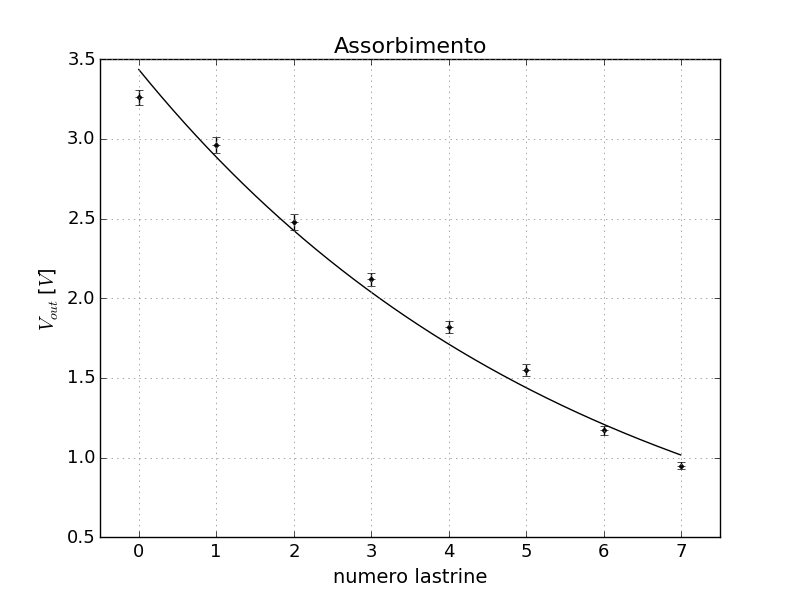
\includegraphics[scale=0.45]{plot-exp1.png}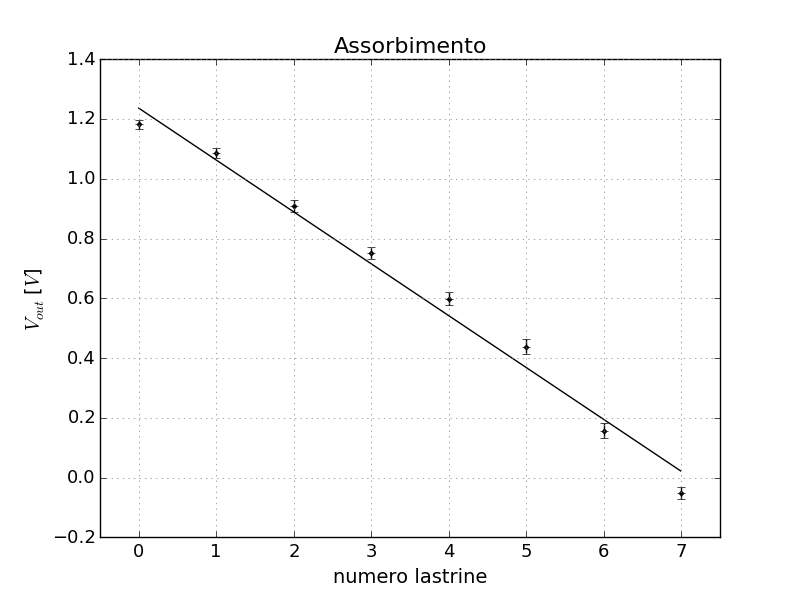
\includegraphics[scale=0.45]{plot-lin1.png}
\caption{A sinistra grafico del fit esponenziale mentre a destra di quello lineare.\label{plot1}}
\end{figure}


\subparagraph{Sfasatore di 90\degree e sfasatore variabile}
I circuiti relativi sono quelli in figura \ref{fig:sfasatori}. L'ingresso S1 è ancora collegato all'uscita del generatore di funzioni. Abbiamo regolato il trimmer P1 in modo da ottenere in S2 la stessa forma d'onda dell'ingresso sfasata di 90\degree (figura \ref{osc:sfasamento}). In S3 l'uscita sarà un'onda quadra e abbiamo regolato il trimmer P3 in modo che il \emph{duty cycle} fosse pari al 50\% (ciò è stato verificato con l'opportuna funzione dell'oscilloscopio, vedi figura \ref{osc:duty}). Se si agisce sul deviatore si bypassa lo sfasatore quindi all'ingresso dello sfasatore variabile l'onda sarà la stessa dell' ingresso S1.\\
L'analisi dello sfasatore mostra che esso ha una funzione di trasferimento nel dominio di Laplace pari a
\begin{equation}
 G(s) = -\frac{1-s(R_{16} +P_1) C_{4}}{1+s(R_{16} + P_1)C_{4}}
\end{equation}
Si osservi che il guadagno è unitario per tutte le frequenze, quindi il circuito si limita ad aggiungere una fase che può essere scelta calibrando il trimmer $P_1$. Inoltre esiste un solo valore della resistenza di trimmer per cui a $1$kHz si ha uno sfasamento positivo di $\frac{\pi}{2}$.\\
L'analisi del circuito che regola il duty cycle (escludendo il transistor finale) si presenta simile, l'uscita S3 risulta in questo caso essere:
\begin{equation}
v_{out}(s) = \left( \frac{s C_3 (R_{13} + P_2)}{1 + s C_3 (R_{13} + P_2)} \frac{R_{12}}{R_8+P_3} -\frac{1-s(R_{13} +P_2) C_{3}}{1+s(R_{13} + P_2)C_{3}} \right) V_{in}-\frac{R_{12} V_{EE}}{R_8+P_3}
\, \, \, \, \, \, ; V_{EE} = -5V.
\end{equation}
%C'è anche una attenuazione da passa alto
Come si vede l'output presenta un offset costante positivo $-\frac{R_{12} V_{EE}}{R_8+P_3}$ il cui valore massimo risulta essere circa $0.61$V. L'aumento della resistenza $P_3$ si vede che causa una diminuzione anche dell'ampiezza del segnale proporzionale a $V_{in}$. 

\begin{figure}[!htb]
  \centering
  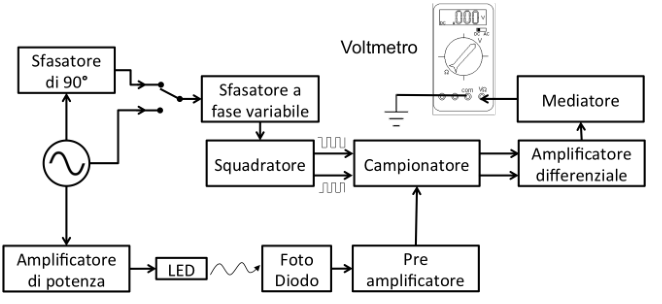
\includegraphics[scale=0.75]{schemablocchi.png}
\caption{Schema a blocchi del circuito Lock-in.\label{fig:schemablocchi}}
\end{figure}

%perchè la abbiamo rimessa?

Il circuito applica anche uno sfasamento rispetto al segnale originario regolabile con $P_2$. L'uscita viene mandata alla base di un transistor la cui polarizzazione è tale da potersi muovere sulla retta di carico solamente  tra la zona di saturazione e quella di interdizione. Il segnale in arrivo sulla base è molto vicino alla tensione di polarizzazione diretta della giunzione BE, dunque la variazione dell'ampiezza della componente oscillante che arriva in base è direttamente legata alla frazione di tempo per cui questo segnale è sufficientemente alto da polarizzare in diretta la giunzione BE mandando quindi il transistor in saturazione. Variare $P_3$ significa modificare dello stesso fattore sia la componente continua che quella oscillante della tensione sulla base, quindi agisce come un coefficiente di dilatazione che permette al segnale di attraversare la barriera di potenziale oltre a cui si ha saturazione per una frazione controllabile del periodo.
Il transistor alternativamente in saturazione e interdizione produce su S3 un'onda quadra (sfasata di $\pi$ rispetto al segnale in base, ma ciò è irrilevante ai fini della nostra analisi).\\
 Abbiamo misurato che si ha un'escursione di fase di $4/5 \pi$ agendo sul trimmer $P_2$. La misura dello sfasamento possibile è stata fatta misurando i tempi intercorrenti fra i punti di 0 dell'onda sinusoidale in S1 e i punti a metà ampiezza  dell'onda quadra in S3.\\
 %vi piace questa specifica?


\begin{figure}[!htb]
  \centering
  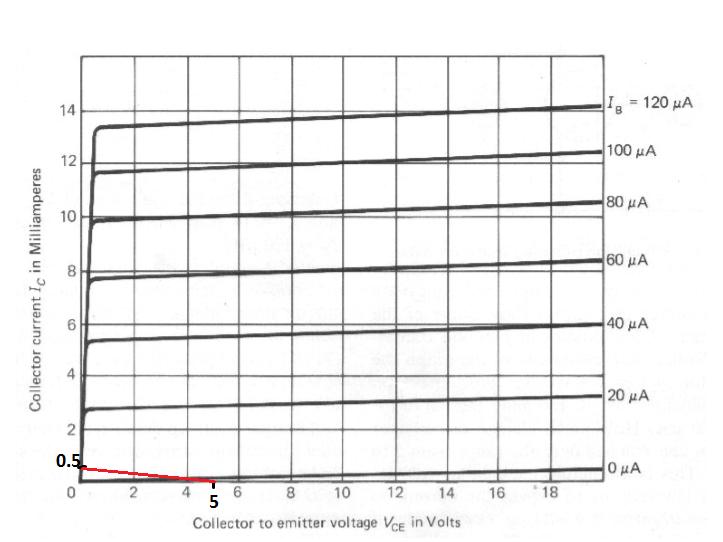
\includegraphics[scale=0.6]{transistorbjt.png}
\caption{Retta di carico del transistor.\label{fig:transistor}}
\end{figure}

Come si vede in figura \ref{fig:transistor} la retta di carico del transistor (in rosso) è molto bassa e non permette mai di entrare veramente in regime attivo. Variare la tensione sulla base commuta quindi il transistor tra gli stati di interdizione e di saturazione.\\

%TODO : Verdficare questa ipotesi e prendere una immagine del segnale il base da schiaffare. Sull'immagin della tenzione in base disegnare la tenzione a cui il transistor viene mandato insaturazione.
%DIRE DEL DUTY CYCLE COME FUNZIONA
%Lo sfasamento dello sfasatore 1 è pi-2arctg(omega/(R16+p1)*C4)
%a basse frequenze lo sfasamento è automaticamente 180gradi
%556/968
%500/980 duty cycle
%escursione di fase con trimmer fase: 4/5pi

 
%ci sono tante immagini di fila, cerco un modo per metterle belline

\begin{figure}[!htb]
  \centering
  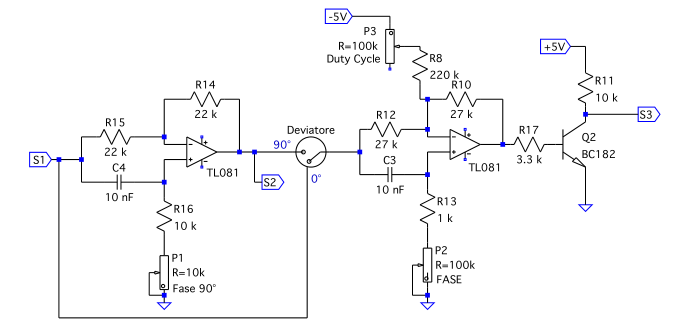
\includegraphics[scale=0.75]{sfasatori.png}
\caption{Schema circuitale dello sfasatore di 90\degree e dello sfasatore variabile.\label{fig:sfasatori}}
\end{figure}

\begin{figure}[!htb]
  \centering
  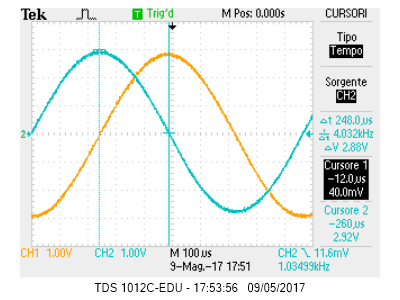
\includegraphics[scale=0.75]{sfasamento90.png}
\caption{Onda S1 in canale 1 e onda S2 in canale 2 sfasate di 90\degree.\label{osc:sfasamento}}
\end{figure}

\begin{figure}[!htb]
\centering
  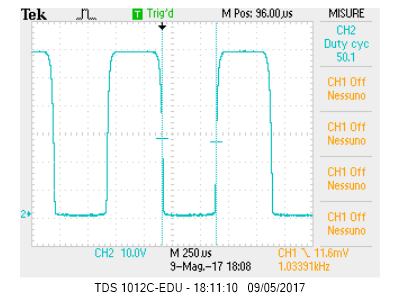
\includegraphics[scale=0.75]{dutycycle50.png}
\caption{Forma d'onda in S3 con duty cycle pari al 50\%. 
\label{osc:duty}}
\end{figure}

\begin{figure}[!htb]
  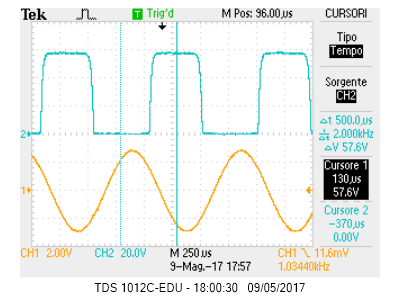
\includegraphics[scale=0.75]{deviatore0.png}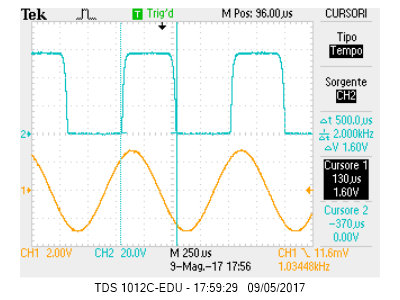
\includegraphics[scale=0.75]{deviatore90.png}
\caption{Forma d'onda in S3, a sinistra con deviatore a 0\degree, a destra con deviatore a 90\degree.\label{osc:dev}}
\end{figure}

\subparagraph{Squadratore e campionatore}
Abbiamo montato i circuiti in figura \ref{fig:sqadratore-campionatore}. Ricordiamo che S3 corrisponde all'onda quadra in uscita dallo sfasatore variabile; questo viene inviato ai due NOT U1 e U2 (che hanno la funzione di rendere più squadrato il segnale), quindi il segnale S4 e il suo negato S5 vengono mandati al campionatore realizzato con un circuito integrato contenente interruttori MOSFET. Seguendo la logica del circuito in figura \ref{fig:sqadratore-campionatore} si vede che S4 e S5 selezionano alternativamente l'uscita S8 o S7 su cui mandare il segnale S6. L'uscita che non lo riceve viene in quel semiperiodo messa a terra.
Cambiando la posizione del deviatore si varia la fase dell'onda che controlla gli interruttori rispetto al segnale da campionare: in questo modo si ottengono segnali con stesso segno (S4 in fase con S1), o a media nulla (S4 sfasato di $90\circ$ rispetto a S1)\\
In figura \ref{osc:s4s5} si osservano i segnali S4 e S5 in opposizione di fase, come atteso, mentre in figura \ref{osc:S7S8} si trovano le forme d'onda S7 e S8 nelle due posizioni del deviatore. In queste ultime due immagini si nota una modulazione dovuta al rumore, infatti in figura \ref{osc:rumore50hz} si osserva rumore a $\simeq 50\,\mbox{Hz}$, che è la frequenza della luce ambientale fornita dalle lampadine. %Fede qui volevi commentare?
Un'ulteriore osservazione riguarda i picchi dei segnali S7 e S8: pensiamo che siano dovuti a una regolazione non perfetta delle fasi o a un ritardo nella propagazione del segnale.

\begin{figure}[!htb]
  \centering
  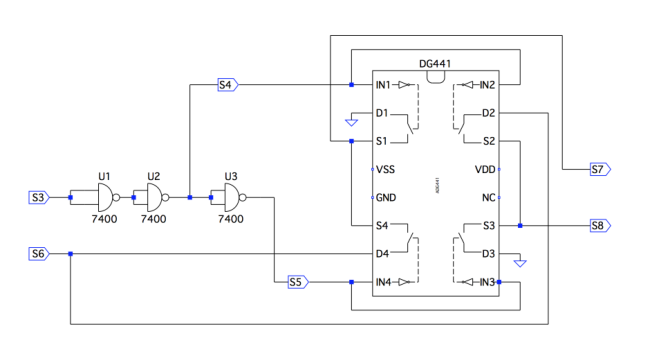
\includegraphics[scale=0.75]{sqadratore-campionatore.png}
\caption{Schema circuitale dello squadratore e del campionatore.\label{fig:sqadratore-campionatore}}
\end{figure}

\begin{figure}[!htb]
  \centering
  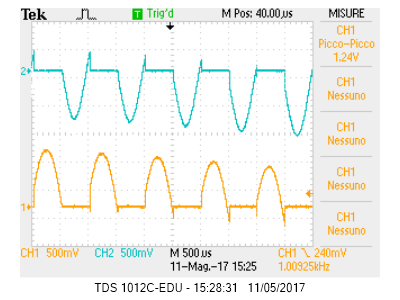
\includegraphics[scale=0.75]{dev0ch1S8-ch2S7.png}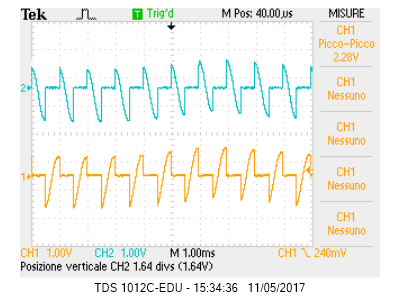
\includegraphics[scale=0.75]{dev90ch1S8-ch2S7.png}
\caption{Onda S8 in canale 1 e S7 in canale 2. Nell'immagine a sinistra il deviatore è collegato a 0\degree mentre in quella a destra a 90\degree . Si nota la modulazione indotta dal rumore a bassa frequenza.\label{osc:S7S8}}
\end{figure}

\begin{figure}[!htb]
  \centering
  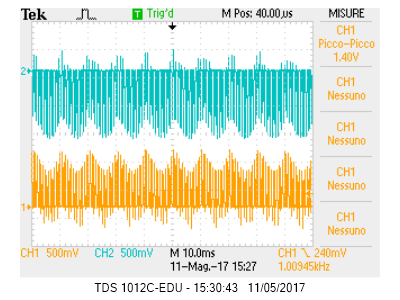
\includegraphics[scale=0.75]{perFedech1S8-ch2S7.png}
\caption{Onda S8 in canale 1 e S7 in canale 2. Rumore a bassa frequenza $\simeq 50\,\mbox{Hz}$.\label{osc:rumore50hz}}
\end{figure}


\subparagraph{Amplificatore differenziale e mediatore}
Infine abbiamo realizzato il circuito in figura \ref{fig:amplificatorediff-mediatore}. Le onde agli ingressi S7 e S8 sono sommate dall'amplificatore differenziale, il quale amplifica la differenza, così da ottenere un output di segno definito o a media nulla, a seconda della posizione del deviatore. In figura \ref{osc:devS9} si trova il segnale S9 per le due posizioni del deviatore, i risultati sono in accordo con quanto detto precedentemente.
Infine due integratori (uno RC e l'altro con OpAmp) rendono continuo il segnale. Le frequenze di taglio di entrambi sono dell'ordine delle decine di Hz, dunque per il segnale a $1\,\mbox{kHz}$ funzionano bene come integratori.% Il segnale mediato è negativo perchè S8 è collegato all'ingresso non invertente dell'OpAmp, infatti scambiando S7 e S8 il segnale risulta positivo. MI ricordo di questa cosa in lab, ma dalle figure che abbiamo messo non sembra che il segnale S9 possa avere media negativa!
 Prima di effettuare le misure di tensione abbiamo posto il deviatore a 0\degree e collegato l'uscita al multimetro digitale, quindi abbiamo regolato il trimmer $P_2$ in modo da avere una tensione nulla per una delle due posizioni del deviatore. Inizialmente abbiamo provato ad annullare il segnale con il deviatore nella posizione 90\degree ma in questo modo non si riusciva per nessunia posizone del potenziometro ad annullare la tensione in uscita a causa della limitata escursione di fase. $V=0.0\pm0.1\,\mbox{V}$. Si è quindi posizionato $P_2$ in modo che fosse nullo il segnale nella posizione a 0\degree (verificato tramite oscilloscopio e multimetro digitale in continua). Abbiamo quindi riacquisito le immagini dei segnali: in figura \ref{osc:S9(zero)} si osserva la forma d'onda S9 nelle due configurazioni del deviatore e anche in questo caso si nota la modulazione indotta dal rumore.

\begin{figure}[!htb]
  \centering
  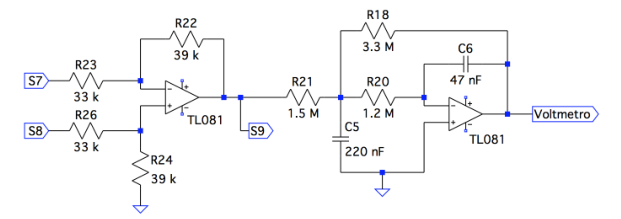
\includegraphics[scale=0.75]{amplificatorediff-mediatore.png}
\caption{Schema a blocchi del circuito Lock-in.\label{fig:amplificatorediff-mediatore}}
\end{figure}

\begin{figure}[!htb]
  \centering
  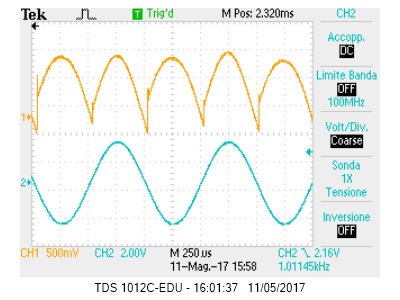
\includegraphics[scale=0.45]{dev0ch1S9-ch2S1.png}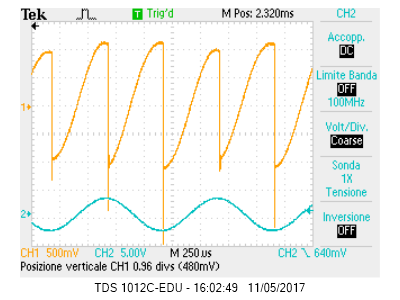
\includegraphics[scale=0.45]{dev90ch1S9-ch2S1.png}
\caption{La forma d'onda S1 (dal generatore di funzioni) è in canale 2, mentre S9 in canale 1. A sinistra il deviatore è a 0\degree, nella figura a destra è a 90\degree. \label{osc:devS9}}
\end{figure}

\begin{figure}[!htb]
  \centering
  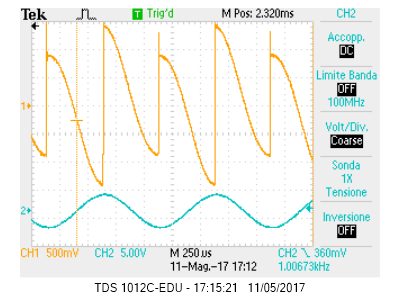
\includegraphics[scale=0.45]{dev0ch1S9-ch2S1(zero).png}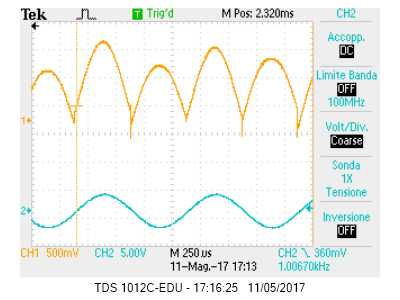
\includegraphics[scale=0.45]{dev90ch1S9-ch2S1(zero).png}
\caption{La forma d'onda S1 (dal generatore di funzioni) è in canale 2, mentre S9 in canale 1. A sinistra il deviatore è a 0\degree, nella figura a destra è a 90\degree. \label{osc:devS9}}
\end{figure}

\section{Presa dati}
Dopo aver settato il segnale con il deviatore a 0\degree su 0, si è posto il deviatore nella posizione 90\degree per effettuare le misure di tensione in funzione del numero di lastrine di Mylar.
Le misure delle tensioni sono state prese tramite multimetro. Durante la presa dati, si è verificato periodicamente (ogni 5 lastrine), che il segnale con 0 lastrine fosse sempre lo stesso. I dati sono presenti in tabella \ref{tab:abs2}. Come in precedenza abbiamo eseguito un fit esponenziale e uno lineare. Dal fit esponenziale (vedi grafico a sinistra della figura \ref{plot2}) abbiamo ottenuto i seguenti parametri: $n_0= 1.388\pm 0.001$, $V_0=6.355\pm0.006\,\mbox{V}$ ma un $\chi^2_{rid}$ molto alto, $x_{ass}=0.208\pm0.001{mm}$. Dal fit lineare (vedi grafico a destra della figura \ref{plot2}) abbiamo ottenuto $a=-0.155\pm0.001$, $b=0.322\pm0.004$ e $\chi^2_{rid}=2.6$, quindi $n_0= 6.45\pm 0.04$, $V_0=1.38\pm0.02\,\mbox{V}$, $x_{ass}=0.967\pm0.006{mm}$.

\begin{table}
\centering
\begin{tabular}{|c|c|c|}
\hline
n	&	$V_{out}\,\mbox{[V]}$	&	$\Delta V\,\mbox{[V]}$\\
\hline
0  & -1.40 & 0.01\\
\hline
1   &-1.19  &0.01\\
\hline
2   &-1.00  &0.01\\
\hline
3   &-0.86  &0.01\\
\hline
4   &-0.72  &0.01\\
\hline
5   &-0.64  &0.01\\
\hline
6   &-0.545  &0.005\\
\hline
7   &-0.460  &0.005\\
\hline
8   &-0.393  &0.004\\
\hline
9   &-0.340  &0.003\\
\hline
10  &-0.300  &0.003\\
\hline
11  &-0.256  &0.003\\
\hline
\end{tabular}
\caption{Presa dati della tensione in uscita al circuito Lock-in.\label{tab:abs2}}
\end{table}

\begin{figure}[!htb]
  \centering
  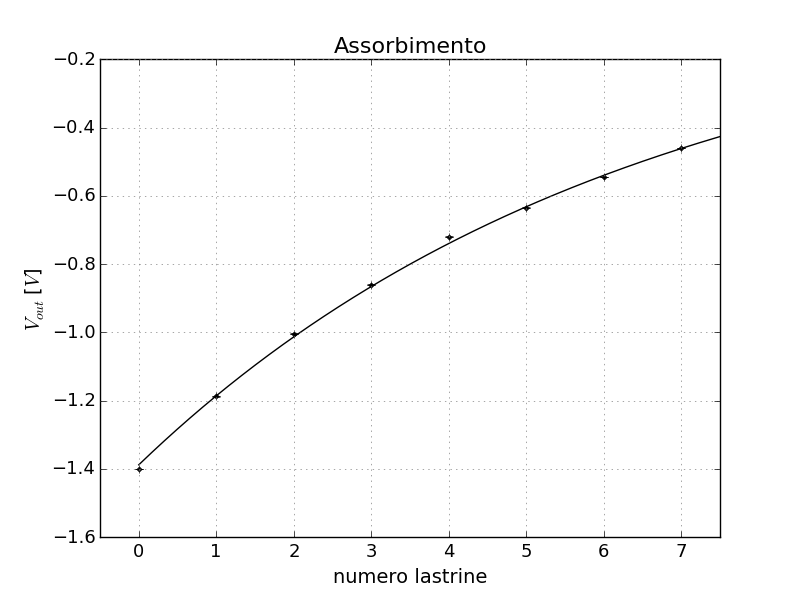
\includegraphics[scale=0.45]{plot-exp2.png}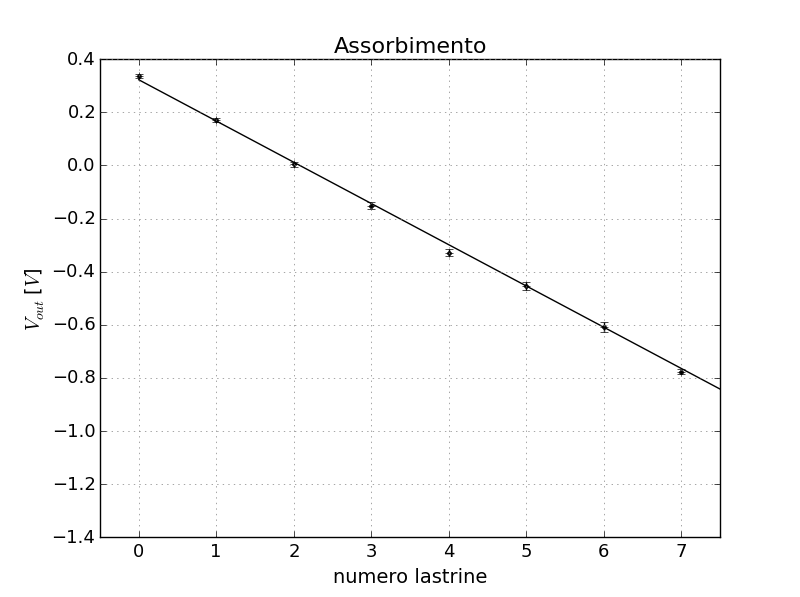
\includegraphics[scale=0.45]{plot-lin2.png}
\caption{A sinistra grafico del fit esponenziale mentre a destra di quello lineare.\label{plot2}}
\end{figure}

\section{Conclusioni}

Le misure eseguite con lock-in risultano non affette da rumore in maniera significativa, pertanto l'incertezza associata è solo strumentale. Nelle misure senza lock-in si aveva una incertezza non solo strumentale, ma dovuta anche al fatto che il rumore spostava significativamente i massimi dei segnali. I dati inoltre sono in maggiore accordo con l'andamento previsto rispetto ai dati presi senza lock-in: infatti nel primo caso si ha un $\chi_{rid} ^2 = $ ,  migliore che nel secondo caso.%specificare quanto è 
 


\end{document}